\begin{frame}
	\frametitle{数学分级考试讲评}
	\linespread{1.2}
	\begin{center}
		\resizebox{!}{5.5cm}{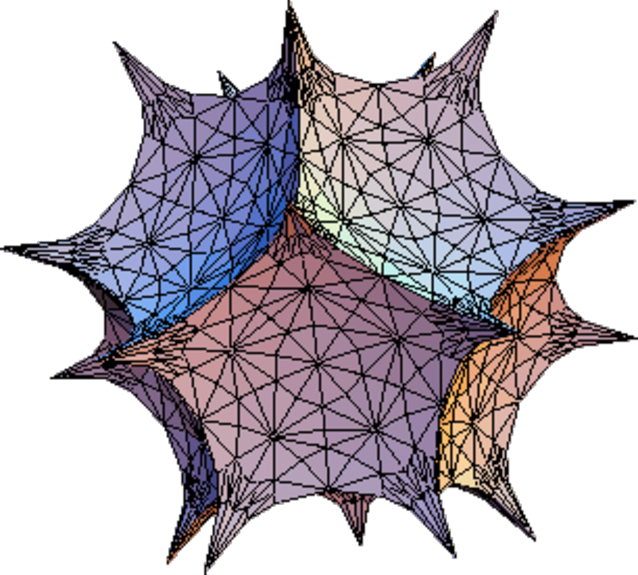
\includegraphics{./images/ch1/hyperball.pdf}}
% 		\resizebox{!}{7.2cm}{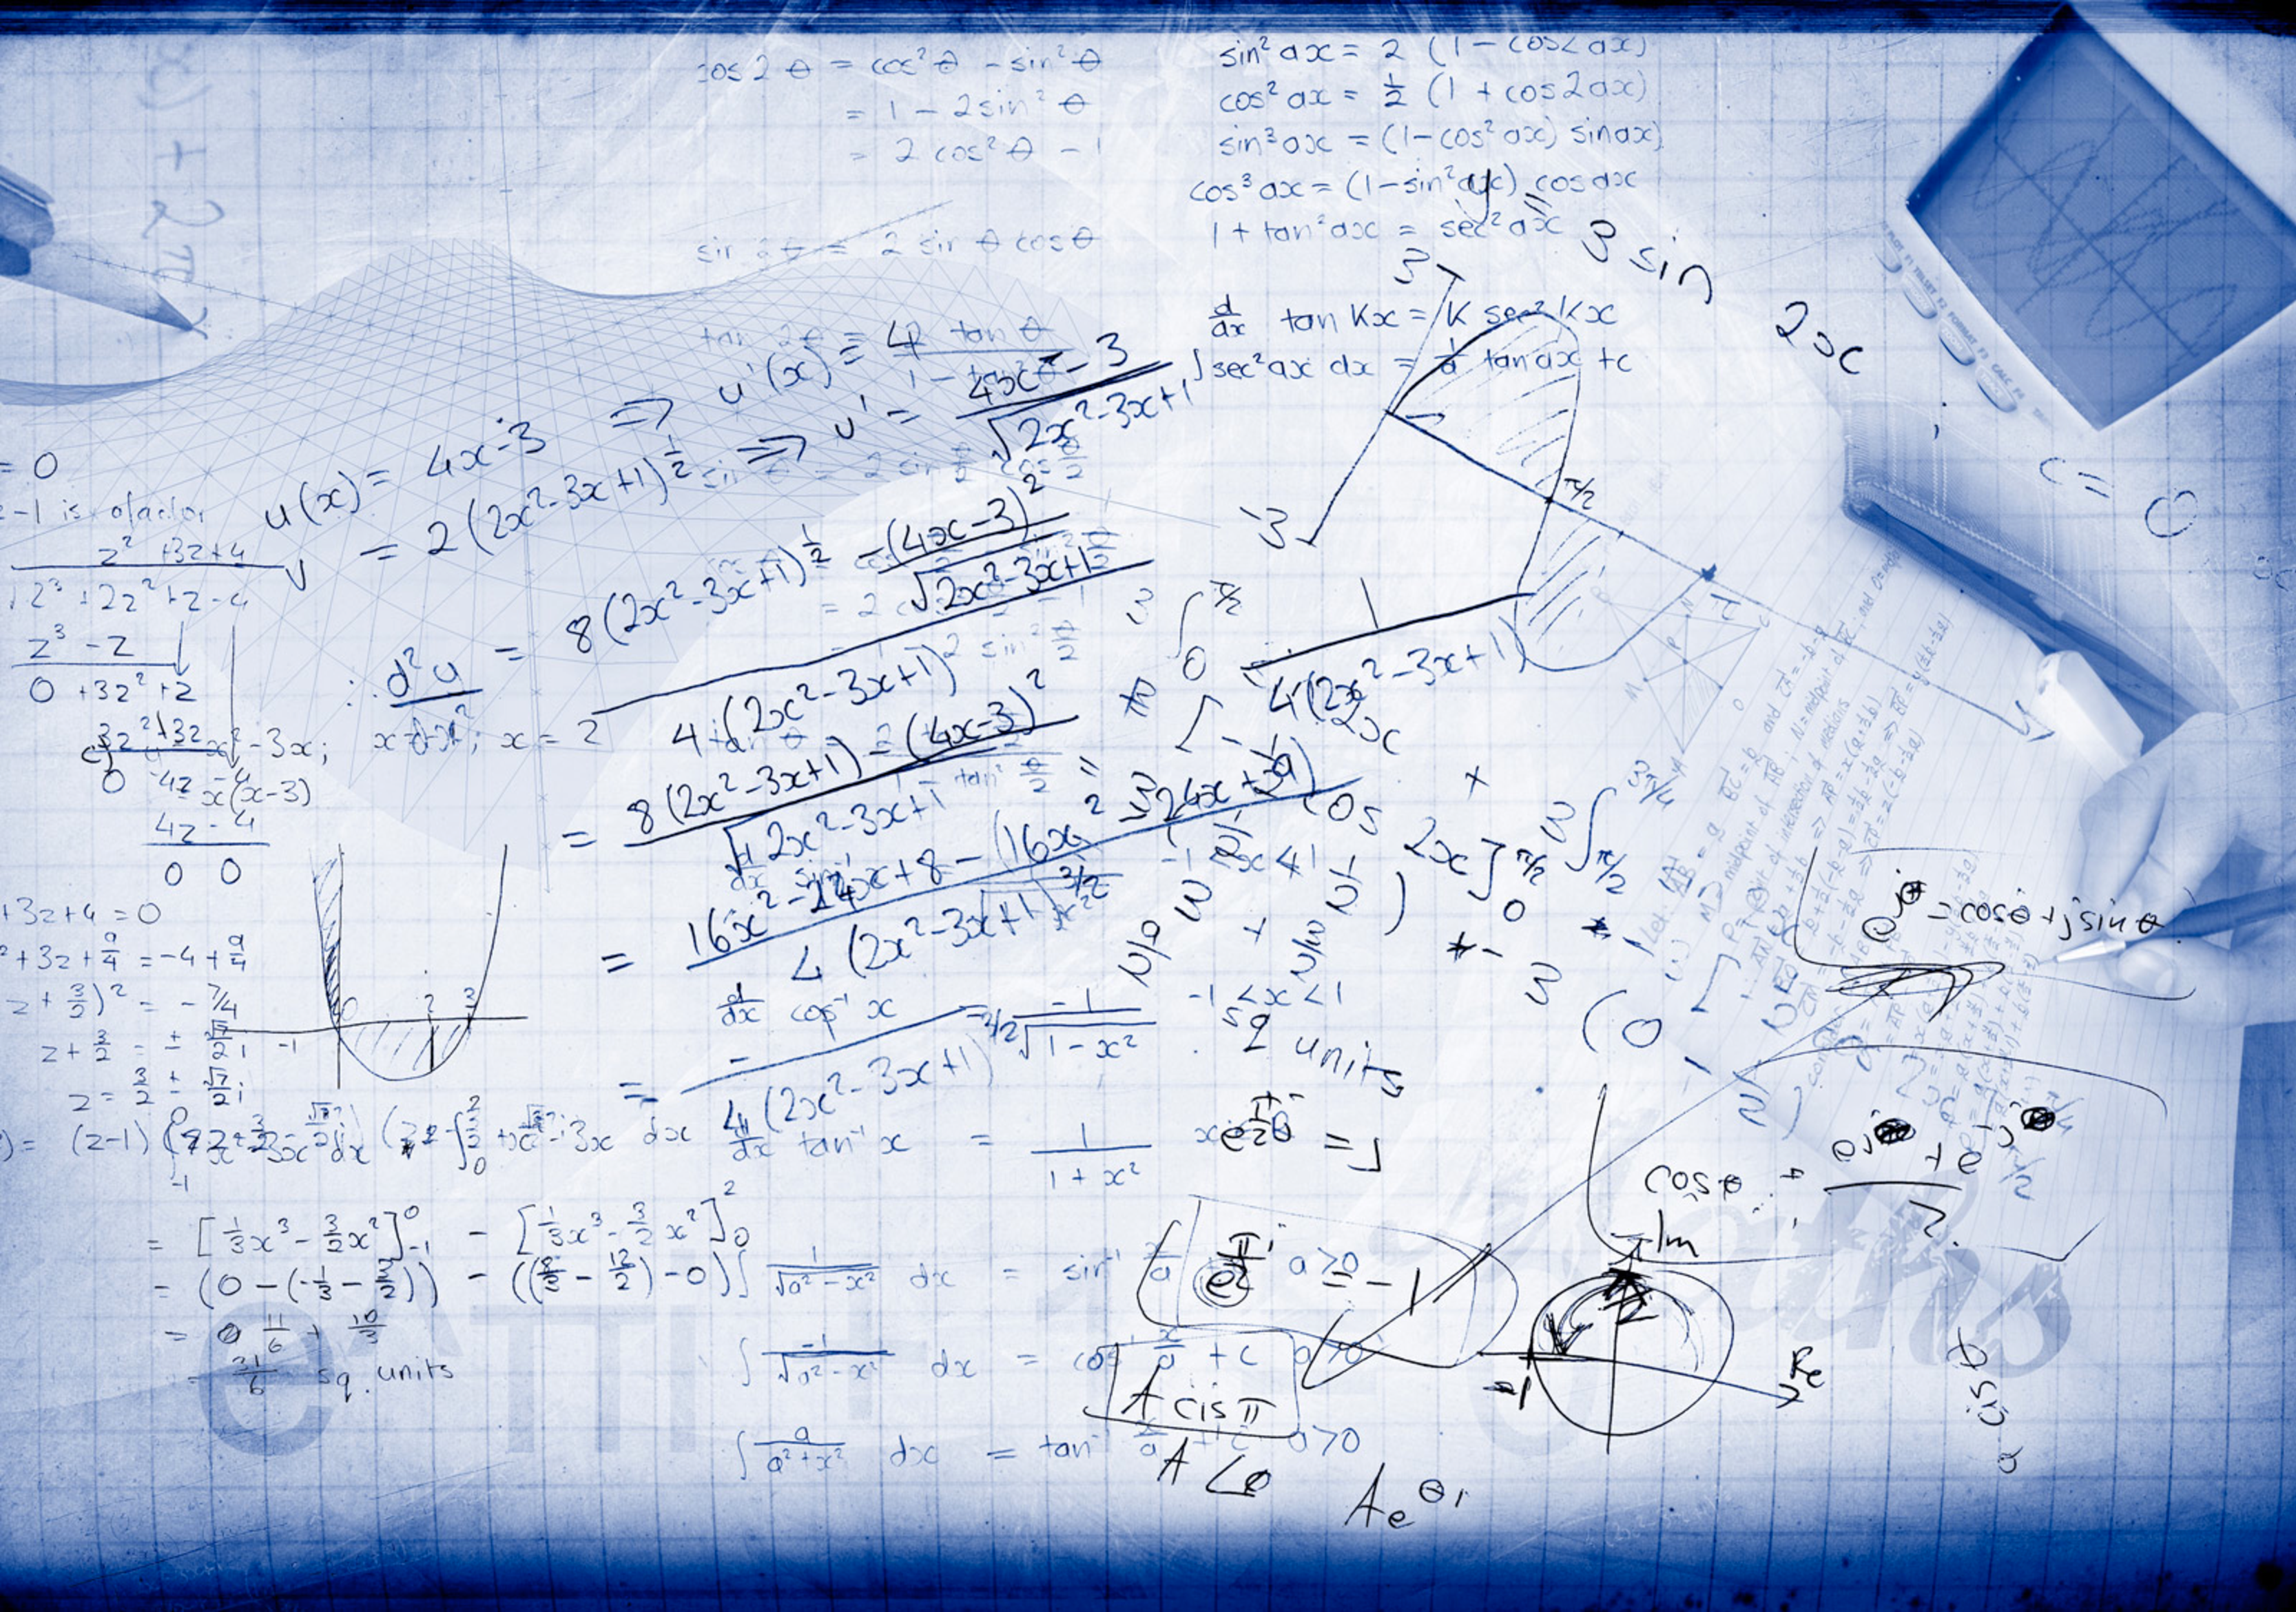
\includegraphics{./images/ch1/math.pdf}}
	\end{center}
\end{frame}

\begin{frame}
	\linespread{1.2}
	\begin{exampleblock}{{\bf 一、简答题(每题6分)}\hfill {\b 10.9}}\pause
		\begin{enumerate}
		  \item 求极限$\lim\limits_{n\to\infty}\left(1-\df 1{2^2}\right)\left(1-\df
		  1{3^2}\right)\cdots\left(1-\df 1{n^2}\right)$。\pause
		  \bigskip
		  \item 设$x_1=1,\;x_2=2,\;x_{n+1}=\df{x_n+x_{n-1}}2\,(n=1,2,$ $\ldots)$,
		  试写出数列$\{x_n\}$的通项公式,并求极限$\lim\limits_{n\to\infty}x_n$。
		\end{enumerate}
	\end{exampleblock}
\end{frame}

\begin{frame}
	\linespread{1.3}
	\begin{exampleblock}{{\bf 一、简答题(每题6分)}\hfill {\b 10.9}}
		\begin{enumerate}
		  \addtocounter{enumi}{2}
		  \item 设映射$f:\mathbb{N}\to\mathbb{N}$满足对所有正整数$n$,恒有$f(n+1)>f(n)$,且
		  $f(f(n))=3n$,求$f(1),\,f(2)$及$f(3^n)\,(n=1,2,\ldots)$。\pause
		  \bigskip
		  \item 设$B$为长、宽、高分别为$L,\,W,\,H$的长方体,现构造一新的立体图形$S$,使$S$由与
		  $B$的距离不超过$1$的所有点组成,求立体$S$的体积。
		\end{enumerate}
	\end{exampleblock}
\end{frame}

\begin{frame}
	\linespread{1.3}
	\begin{exampleblock}{{\bf 二、(12分)}\hfill{\b 7.6}}
		 如图放置的边长为$1$的正方形$ABCD$沿$x$轴滚动(包含沿$x$轴正负两个方向滚动;沿
		$x$轴正向滚动是指先以$A$为中心顺时针旋转,当$B$落在$x$轴上时,再以$B$为中心顺时针旋转,如此继续。沿
		$x$轴负向滚动类似),设顶点$C(x,y)$的轨迹方程为$y=f(x)$。\pause
		\begin{enumerate}
		  \item 写出$f(x)$在区间$[0,4]$上的表达式;\pause
		  \item 写出$f(x)$在$[2011,2012]$上的表达式;\pause
		  \item 求定积分$\dint_{-4}^4f(x)dx$。
		\end{enumerate}
% 		\begin{center}
% 			\resizebox{!}{4cm}{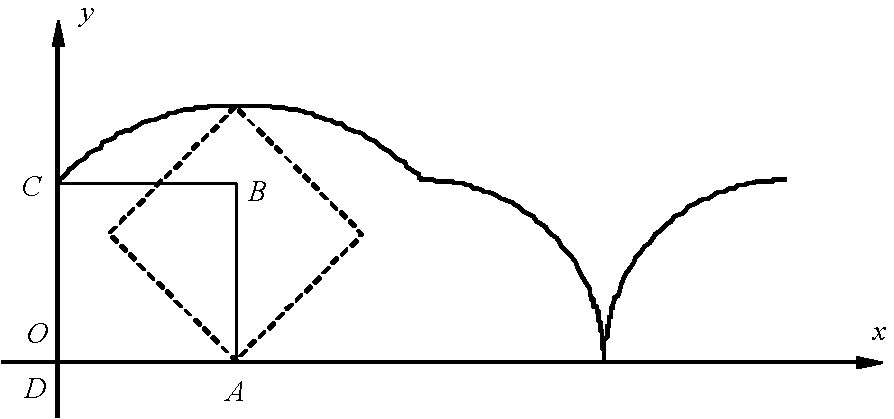
\includegraphics{./images/ch1/abcdRoll.pdf}}
% 		\end{center}
	\end{exampleblock}
\end{frame}

\begin{frame}
	\linespread{1.2}
	\begin{exampleblock}{{\bf 二、(12分)}\hfill{\b 7.6}}
		\begin{enumerate}
		  \item 写出$f(x)$在区间$[0,4]$上的表达式;
		  \item 写出$f(x)$在$[2011,2012]$上的表达式;
		  \item 求定积分$\dint_{-4}^4f(x)dx$。
		\end{enumerate}
	\end{exampleblock}\pause
	\begin{center}
		\resizebox{!}{4cm}{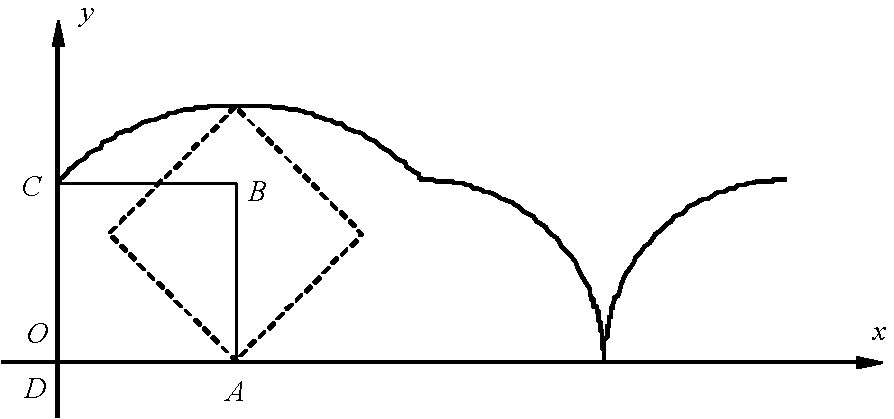
\includegraphics{./images/ch1/abcdRoll.pdf}}
	\end{center}
\end{frame}

\begin{frame}
	\linespread{1.5}
	\begin{exampleblock}{{\bf 三、(12分)}\hfill{\b 5.7}}
		甲袋中有$1$个黑球$2$个白球,乙袋中有$3$个白球,每次从袋中各任取一球,交换后
		放入另一个袋中。求交换$n$次后,黑球仍在甲袋中的概率。
	\end{exampleblock}
\end{frame}

\begin{frame}
	\linespread{1.2}
	\begin{exampleblock}{{\bf 四、(12分)}\hfill{\b 8.0}}
		设$a_1,\,a_2$是不相同的整数,
		$$f_1(x)=(x-a_1)(x-a_2)-1,$$
		$$f_2(x)=(x-a_1)(x-a_2)+1,$$
		\vspace{-1em}\pause
		\begin{enumerate}
		  \item 证明:方程$f_1(x)=0$没有整数根;\pause
		  \item 给出方程$f_2(x)=0$有整数根的充分必要条件。
		\end{enumerate}
	\end{exampleblock}
\end{frame}

\begin{frame}
	\linespread{1.0}
	\begin{exampleblock}{{\bf 五、(14分)}\hfill\hfill{\b 3.9}}
		设$B,\,C$是我军的两个前沿观察哨所,$A$是我军的炮兵阵地,$A$位于$B$的正东,两者
		相距$6$千米,$C$位于$B$的正北偏西$30$度,相距$4$千米。某天凌晨$4$点$15$分$21$秒,$A$发现某一信号,
		$4$点$15$分$31$秒,$B,\,C$哨所同时发现该信号。经查实此信号发自敌方一观察哨所$P$,指挥部命令$A$对该
		哨所实施打击,已知该信号的传播速度为$0.4$千米每秒。\pause
		\begin{enumerate}
		  \item 计算$A$炮击目标的射程以及炮击的方位角\pause
		  \item 若发射炮弹的初速度为$\ds\sqrt{\df{20\sqrt 3}3}g$,计算从$A$处准确射击的仰角(不计空气阻力)
		\end{enumerate}
	\end{exampleblock}
\end{frame}

\begin{frame}
	\linespread{1.2}
	\begin{exampleblock}{{\bf 六、(16分)}\hfill\hfill{\b 3.2}}
		已知函数$f(x)=\ln\left(1+\df 1x\right)-\df 1{x+a},\,x>0,\, a\geq 0$\pause
		\begin{enumerate}
		  \item 讨论函数$f(x)$的单调性,并求其极值点$X(a)$;\pause
		  \item 若极值点在函数$f(x)$的图像上的坐标为$P(X(a),$ $Y(a))$,试讨论点$P$的位置随$a$变化的情况;\pause
		  \item 对于不同的参数,函数$f(x)$对应的图像是否会相交?说明理由;\pause
		  \item 绘出曲线族的大致形状,指出随参数$a$的变化时,曲线形状发生了几次大的变化?
		\end{enumerate}
	\end{exampleblock}
\end{frame}

\begin{frame}
	\linespread{1.2}
	\begin{center}
		\resizebox{!}{6cm}{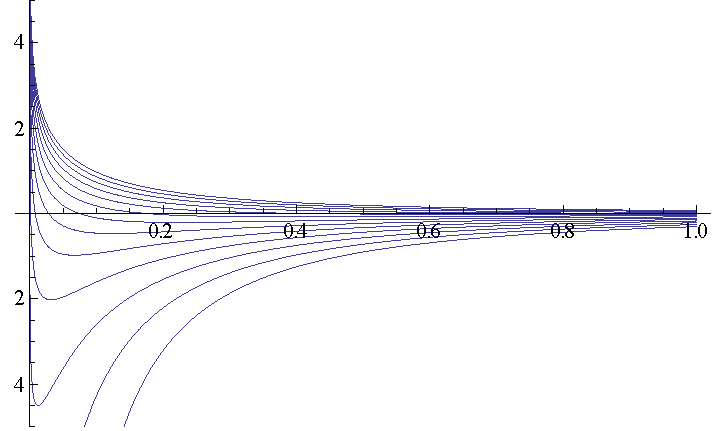
\includegraphics{./images/ch1/fxa.pdf}}
		$$f(x)=\ln\left(1+\df 1x\right)-\df 1{x+a},\,x>0,\, a\geq 0$$
	\end{center}
\end{frame}

\begin{frame}
	\linespread{1.4}
	\begin{exampleblock}{{\bf 七、(10分)}\hfill\hfill{\b 4.8}}
		如果$F'(x)=f(x),\,x\in(a,b)$,则称函数$f(x)$为$F(x)$的导函数,$F(x)$为
		$f(x)$在区间$(a,b)$内的一个原函数。\pause
		\begin{enumerate}
		  \item 问:一个周期函数的导函数是否必为周期函数?一个周期函数的原函数是否必为周期函数?说明理由。\pause
		  \item 试写出函数$f(x)=\df{1+\cos x}{(x+\sin x)^2}$的一个原函数。
		\end{enumerate}
	\end{exampleblock}
\end{frame}

\begin{frame}
% 	\frametitle{数学分级考试讲评}
	\linespread{1.2}
	\begin{center}
% 		\resizebox{!}{5.5cm}{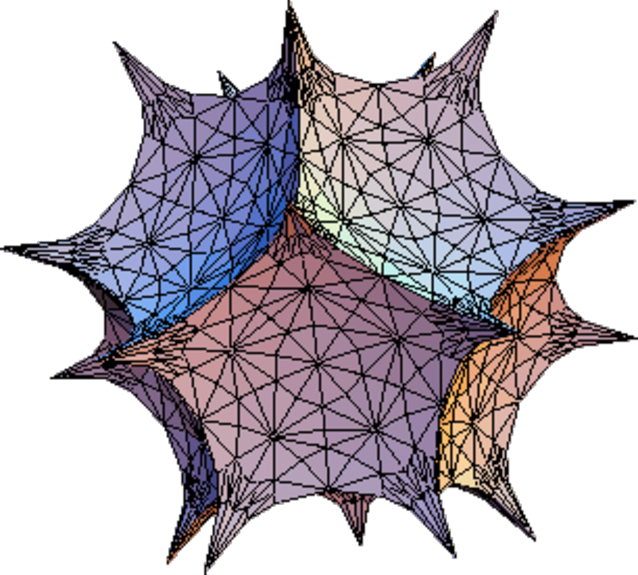
\includegraphics{./images/ch1/hyperball.pdf}}
		\resizebox{!}{8cm}{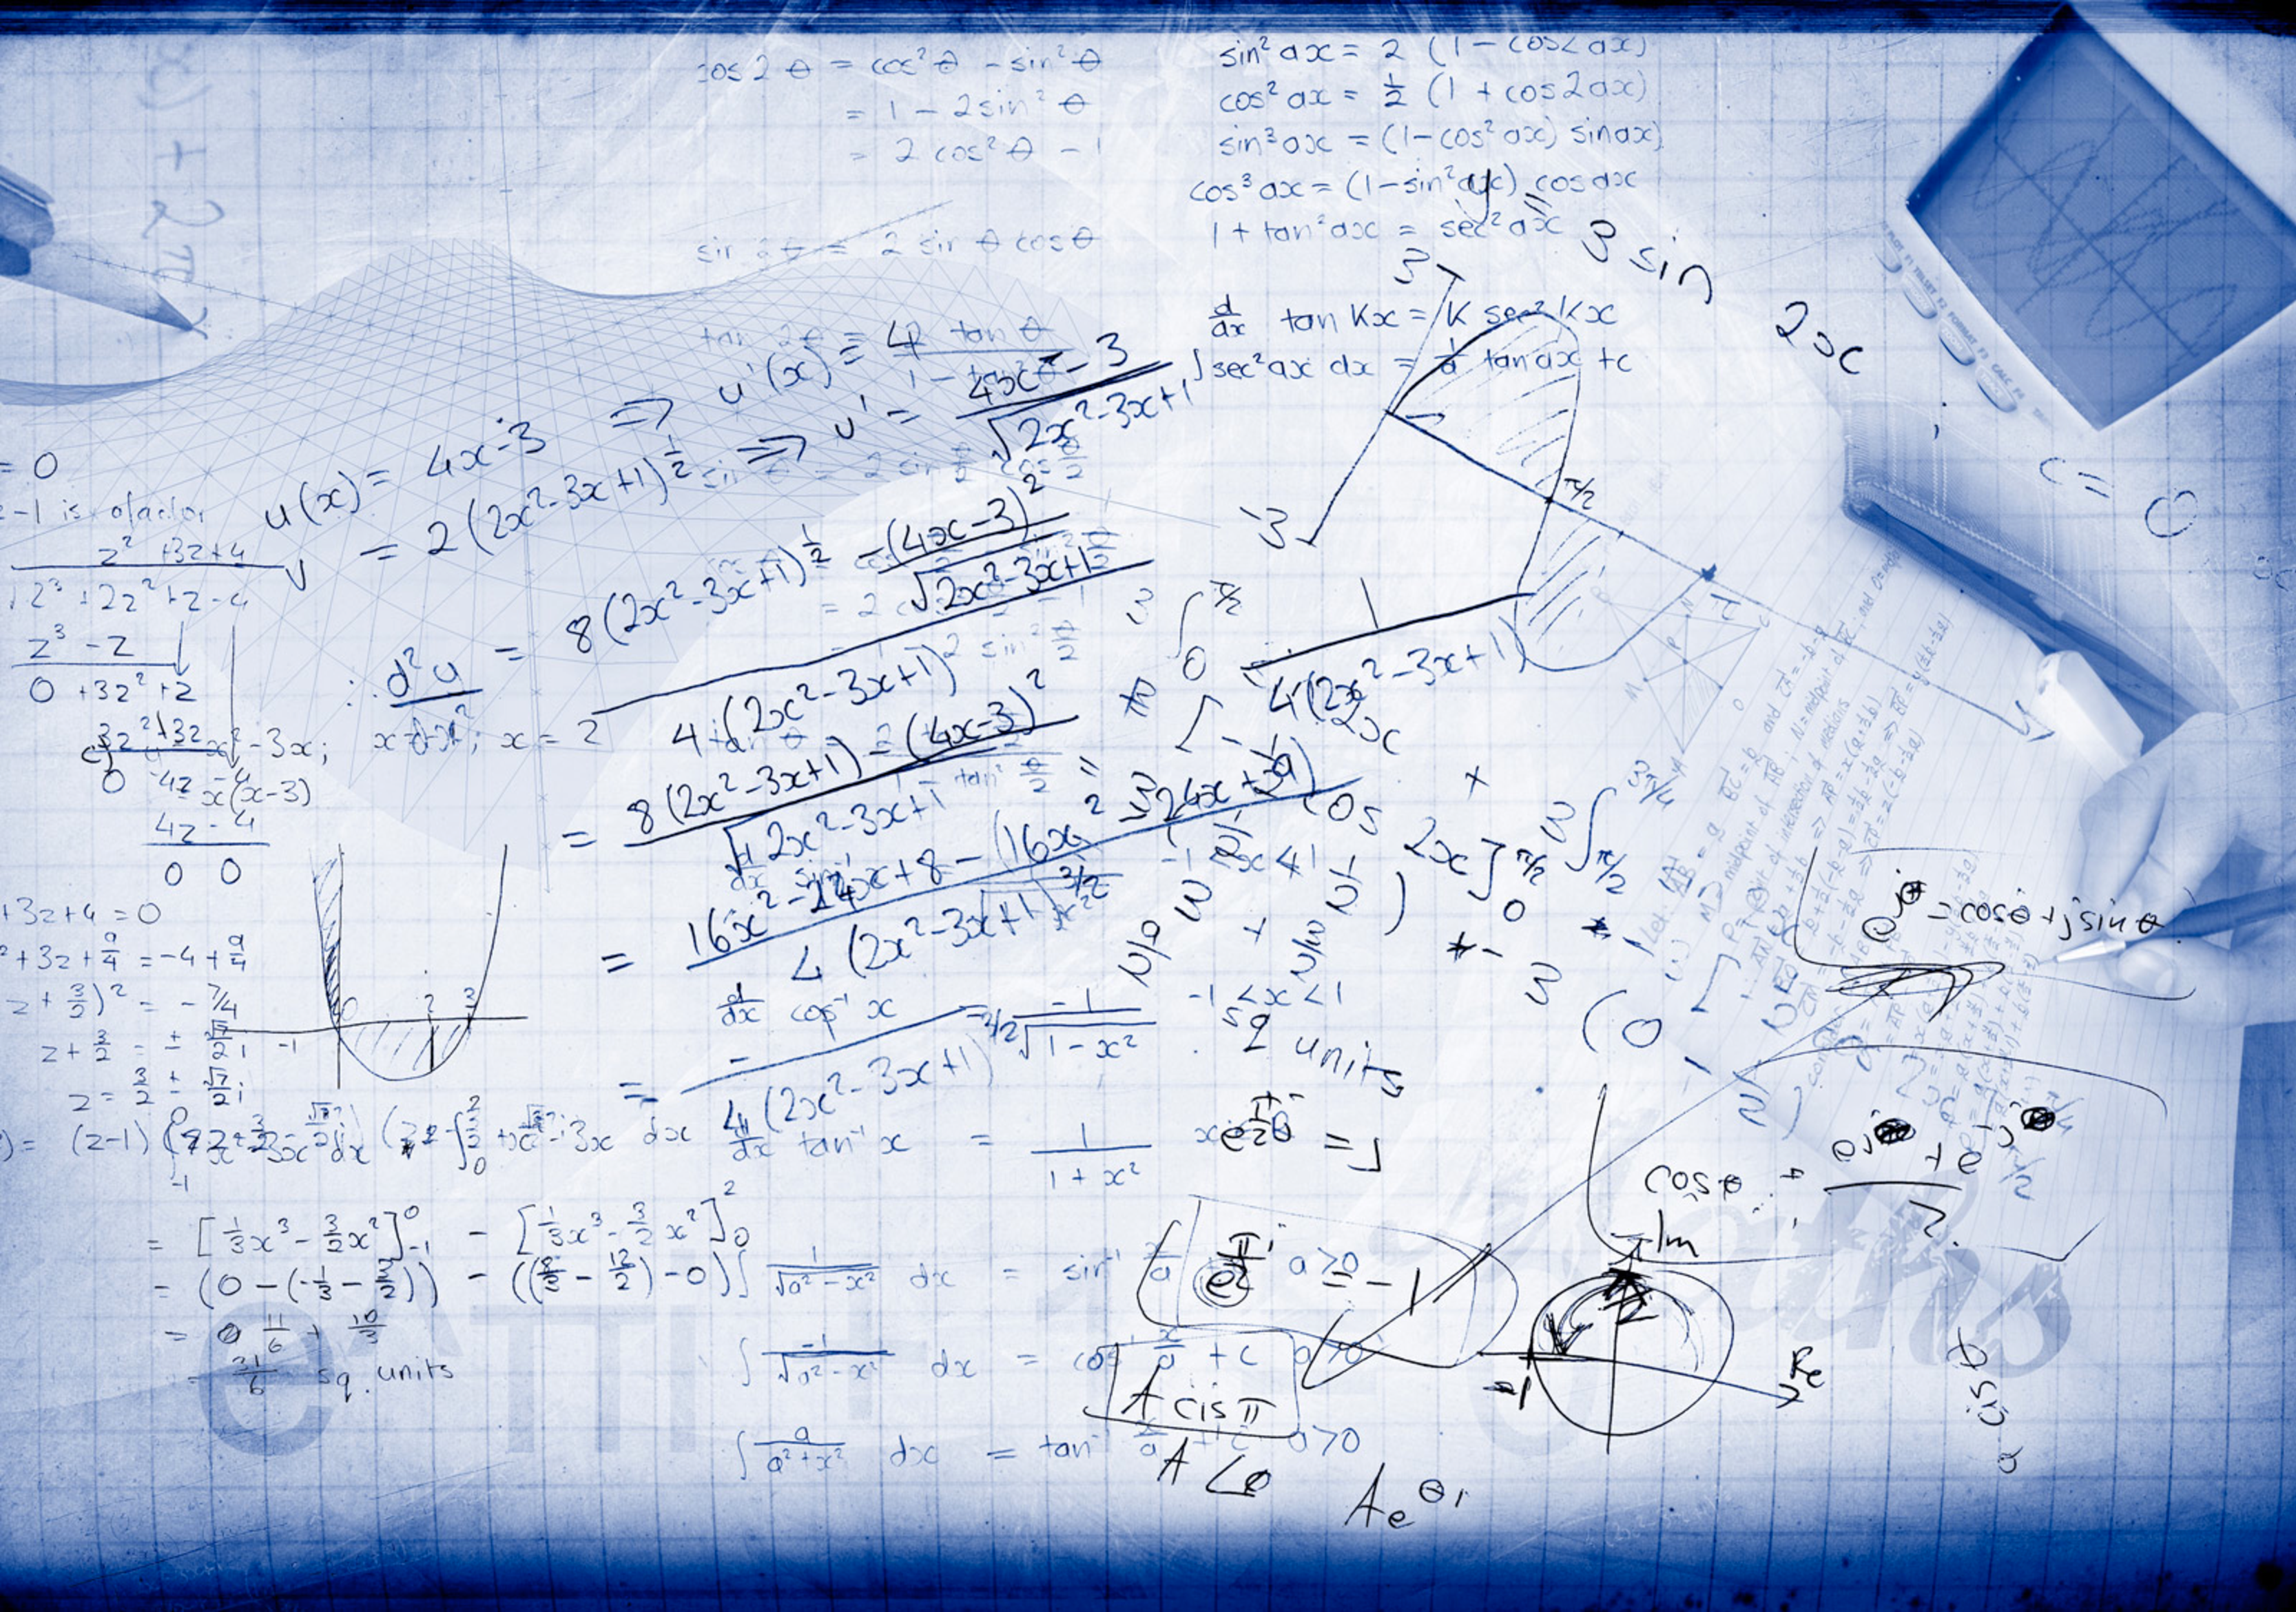
\includegraphics{./images/ch1/math.pdf}}
	\end{center}
\end{frame}